\documentclass[12pt,a4paper]{scrreprt}
\usepackage[utf8]{inputenc}
\usepackage{amsmath}
\usepackage{amsfonts}
\usepackage{amssymb}
\usepackage{todonotes}	
\usepackage[]{graphicx} 


\title{Handbuch \\ Gemeinsame, verteilte Überwachung eines Gebietes auf Eindringlinge}
\author{Dennis Lisiecki, Torsten Kühl}

\begin{document}

\maketitle	%Titelblatt erstellen
\tableofcontents	%Inhaltsverzeichnis erstellen


\chapter{Vorbereitung}
\section{Vorwort}
Willkommen bei Codis und vielen Dank für das Interesse an unserer Lösung eines Überwachungssystems. Codis steht kurz für \textit{Cooperative, Distributed Surveillance}. Wir haben Codis mit dem Ziel begonnen, ein kooperatives System für die Überwachung eines Gebietes zu erstellen, dass für den schmalen Geldbeutel eine veritable alternative zu einem "ausgewachsenem" Überwachungssystem darstellt. Die folgenden Seiten werden Ihnen helfen, einen neuen Raspberry Pi für diese Zwecke vorzubereiten und die Software in Betrieb zu nehmen. Wir möchten darauf hinweisen, dass wir für unser Überwachungssystem das Raspberry Pi B+ Modell empfehlen. Leider war es uns nicht möglich auch andere Modelle zu testen aber der Preisunterschied ist äußerst Marginal und die zusätzlichen USB-Anschlüsse und die damit gewonnene Flexibilität den Aufpreis wert. Generell sollte es allerdings kein Problem darstellen, das System auf einem anderen Modell zu installieren. \\In den nächsten Kapiteln erfahren Sie, welche Teile Sie benötigen, wie Sie Ihr System konfigurieren sollten und wie Sie die Einzelteile zusammensetzen. 

\section{Diese Teile werden benötigt}
\begin{itemize}
\item Raspberry Pi B+
\item SD-Karte
\item Strom für den Raspberry Pi
\item Monitor (für Ersteinrichtung)
\item Tastatur und Maus (für Ersteinrichtung) 
\item Pi NoIR-Kamera
\item PIR-Sensor
\item Ein Paket Kabel
\item Android-Kompatibles Gerät(Handy oder Tablet)
\end{itemize}

\section{Den Raspberry vorbereiten}
Im Folgendem gehen wir davon aus, dass der Raspberry Pi bzw. die SD-Karte bereits mit der aktuellsten Version vom Raspbian-OS ausgestattet ist. Die Größe der SD-Karte sollte ca. 4 GB betragen. Da keine Video- oder Bilddaten aufgezeichnet werden und lediglich das Betriebssystem und dessen Updates auf der SD-Karte Platz finden müssen, benötigen wir für unsere Zwecke keine größere Speicherkarte.\\Um später ohne einen direkt angeschlossenen Monitor arbeiten zu können, empfiehlt sich die Nutzung der Secure Shell, kurz SSH genannt. Durch die Nutzung der SSH-Verbindung ersparen wir uns den Zwang, einen Monitor an den Raspberry Pi anzuschließen und sogar direkt angeschlossene Peripherie wie Maus und Tastatur werden dadurch unnötig. Dadurch ist es möglich, das System an einer schwer zugänglichen Stelle zu platzieren und trotzdem direkten Zugriff auf den Raspberry Pi zu haben. Es ist auch kein Download von Softwarepaketen nötig - SSH ist bereits vorinstalliert und kann sofort verwendet werden. Wie dies geschieht, erklären wir in einem separaten Kapitel in dieser Anleitung. Nur zur Ergänzung sei noch erwähnt, dass auch für diejenigen, die lieber auf einer grafischen Oberfläche arbeiten wollen, eine Lösung existiert. Dazu muss allerdings ein VNC-Server installiert werden. Dieser ermöglicht dann das Arbeiten auf der LXDE - der grafischen Oberfläche von Raspbian. Entsprechende Anleitungen zu der Einrichtung finden sich im Internet. Einzige Voraussetzung für die Nutzung von SSH und VNC ist eine funktionierende Netzwerkanbindung. \\Für die Funktionsweise des Überwachungssystems ist eine funktionierende Netzwerkanbindung ohnehin unablässig und die Ersteinrichtung wird im Folgendem Kapitel kurz erklärt.

\section{WLAN einrichten}
Für unsere Überwachungskamera ist es nützlicher von vornherein einen WLAN-Stick für die Netzwerkanbindung zu nutzen. Dadurch ist man viel flexibler was die Positionierung der Kamera(s) angeht und da keine großen Datenmengen verschickt werden, ist der geringe Datendurchsatz bei Verwendung eines WLAN-Sticks nicht weiter tragisch. Leider ist das Einrichten auch ein wenig komplizierter, als bei der Alternative: Für eine Nutzung mit Kabel reicht es meist, das Lan-Kabel an den Netzwerkanschluss des Raspberry Pi anzuschließen. In den wenigsten Fällen sollte jetzt noch ein Eingreifen nötig sein - sofern der Router im Netzwerk DHCP unterstützt und dem Raspberry Pi erfolgreich eine IP-Adresse zuteilt. Für die Nutzung eines WLAN-Sticks ist leider ein wenig mehr Aufwand vonnöten: Am einfachsten gestaltet sich die Einrichtung über die LXDE, die grafische Oberfläche von Raspbian. Denn dort existiert ein Programm, ebenfalls mit grafischer Oberfläche, welches bei der Ersteinrichtung unterstützt. Das Programm finden Sie im Startmenü unter dem Punkt "Internet" und nennt sich "wpa\_gui". Wenn man den Stick an einen der USB-Anschlüsse angesteckt hat, scannt man das Netzwerk, sucht seinen Router aus der Liste und kann nach Eingabe des Passworts eine Verbindung herstellen. Praktisch: Bei erfolgreicher Verbindung zeigt uns das Programm sofort die IP-Adresse des Raspberry Pi an. Die IP-Adresse ist wichtig für die SSH-Verbindung und kann jetzt schonmal notiert werden. Alternativ kann die Einrichtung auch über die Kommandozeile erfolgen, was für den Laien allerdings (noch) nicht zu empfehlen ist. Hierzu navigieren wir in den Pfad \textit{"/etc/wpa\_supplicant/"} und öffnen mit dem Befehl \textit{"sudo nano wpa\_supplicant.conf"} die Konfigurationsdatei für die Drahtlosverbindung. Hier müssen nun per Hand die Daten für die Konfiguration eingetragen werden. In die Zeile beginnend mit \textit{"ssid="} gehört der Name des Routers in Anführungszeichen eingetragen. In der folgenden Zeile, beginnend mit \textit{"psk="} muss das Passwort für das WLAN eingetragen werden. Die Zeilen sollten dann in etwa so aussehen:\\ \begin{figure}[h] 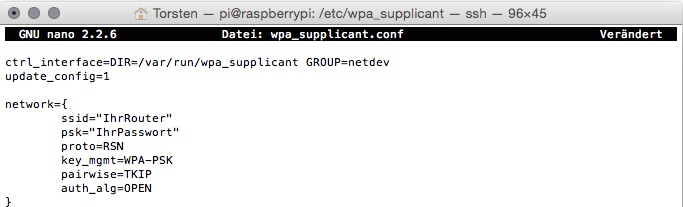
\includegraphics[width=15.8cm]{wpa} \caption{Beispiel für Inhalt der wpa\_supplicant.conf} \end{figure} \\ Um die erfolgreiche Konfiguration zu testen, empfiehlt sich nun zunächst ein kurzer Neustart mittels des Befehls \textit{"sudo reboot"}. Nach dem Neustart kann die IP-Adresse im Terminal oder der Kommandozeile mit dem Befehl \textit{"hostname -I"}ausgelesen werden. Wenn die Einrichtung erfolgreich war, sollte in der folgenden Zeile die aktuelle IP-Adresse des Raspberry Pi angezeigt werden. Jetzt, da wir im besten Fall mit dem Internet verbunden sind, ist es ratsam den Raspberry Pi mit den Befehlen \textit{"sudo apt-get update"} und \textit{"sudo apt-get upgrade"} auf den neuesten Stand zu bringen. Je nach bevorzugter Vorgehensweise, gibt man die Befehle einfach im Terminal oder der Kommandozeile ein. Dadurch werden alle installierten Pakete auf den neuesten Stand angehoben und auch das Betriebssystem aktualisiert.


\section{Zugriff über SSH}
Um nun auf den Raspberry Pi zugreifen zu können, müssen je nach Betriebssystem, von welchem der Zugriff erfolgen soll, andere Wege genommen werden. Bei einem Zugriff von Windows aus empfiehlt sich das Programm \textit{Putty}. Nach dem Download kann über die IP-Adresse der Zugriff erfolgen. \\Der Zugriff von Macintosh- und Linux-Rechnern kommt ohne zusätzliche Software aus. Öffnen Sie dazu das Terminal und geben dort den Befehl \textit{"ssh pi@192.168.2.10"} ein. Dieser Befehl versucht nun eine gesicherte Verbindung zu dem Raspberry Pi mit der IP-Adresse 192.168.2.10 herzustellen und meldet den Benutzer "pi" an. Egal welches Betriebssystem und welche Software verwendet wird, werden Sie vor der erfolgreichen Verbindung noch nach dem Passwort für den Benutzer gefragt, der die Verbindung herstellen möchte. Falls Sie das Passwort für den Standardbenutzer "pi" noch nicht geändert haben sollten, so lautet dieses \textit{raspberrypi}. Falls die Verbindung erfolgreich war, können Sie nun über die Kommandozeile auf dem Raspberry Pi arbeiten. \\ Übrigens lässt sich die Secure Shell auch für die Datenübertragung verwenden: Mit einem Ftp-Client können Sie eine gesicherte Datenübertragung mit dem Raspberry Pi starten. Achten Sie bei dem Verbindungsversuch darauf das sftp-Protokoll zu benutzen und Sie können fleißig Daten verschieben. Die Anmeldedaten sind die gleichen, wie bei der herkömmlichen SSH-Verbindung.

\chapter{Aufbau}
\section{Die Kamera}
 \begin{figure}[h] \centering 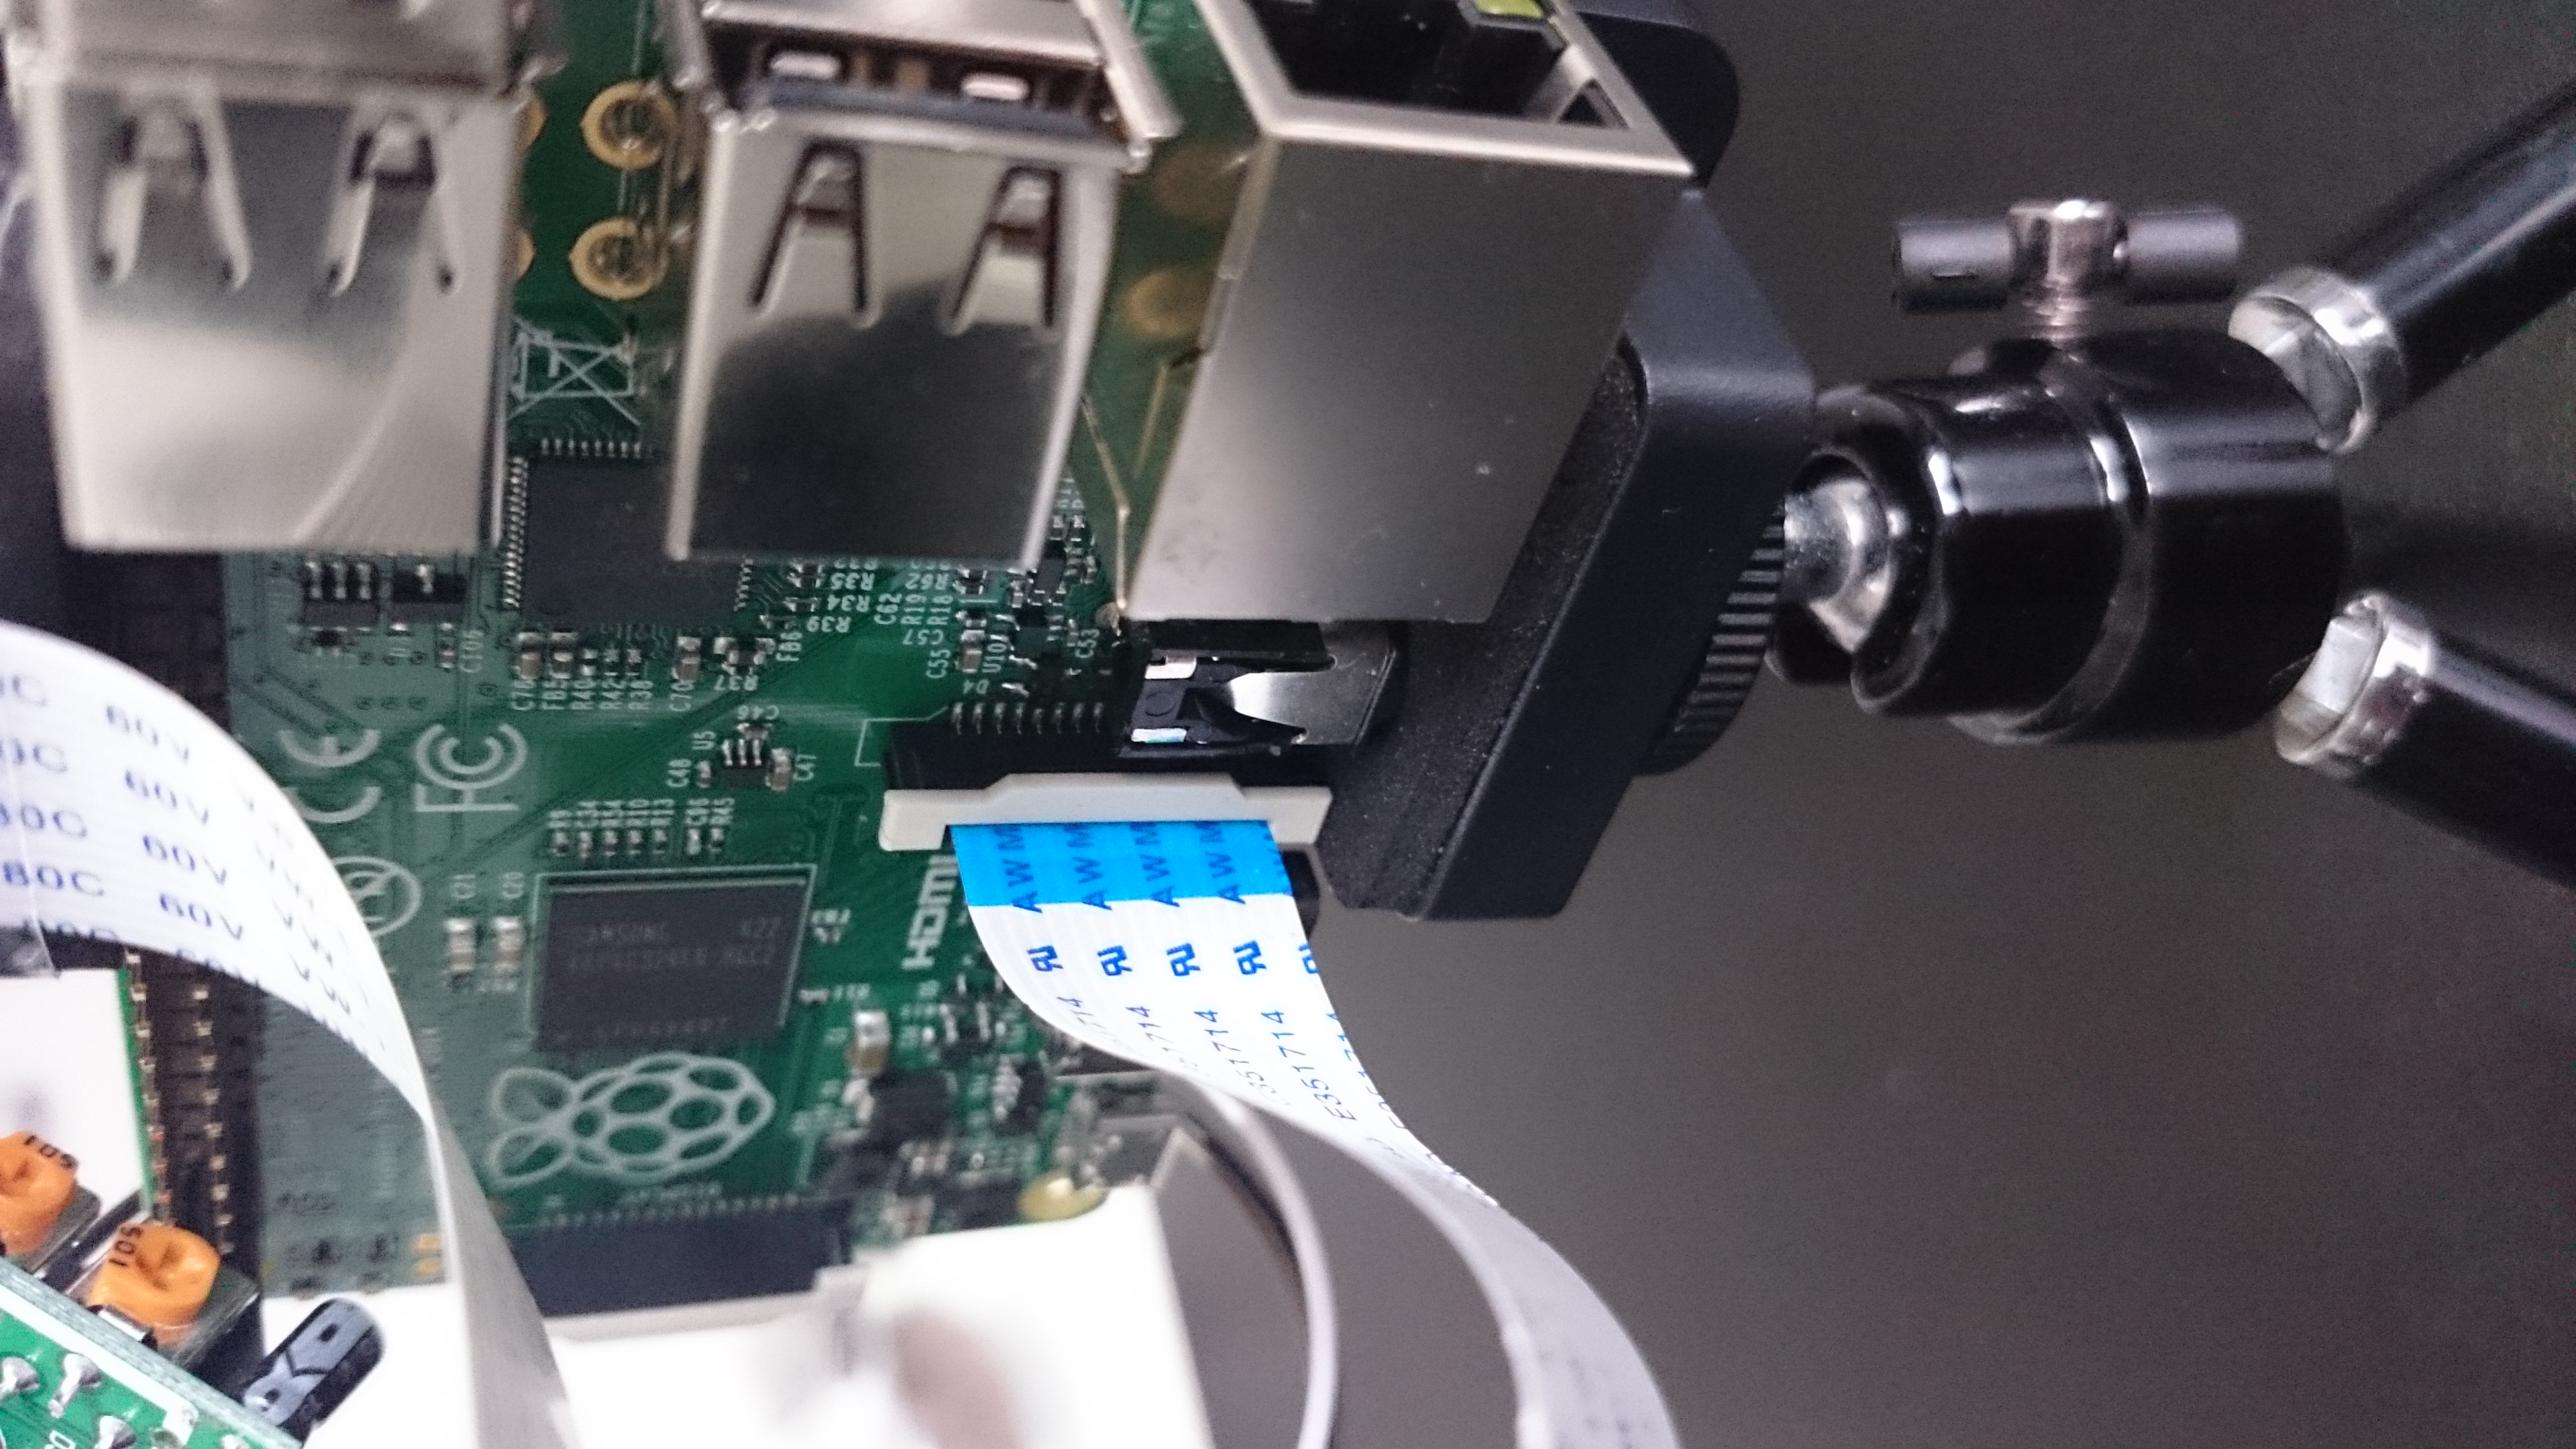
\includegraphics[width=7.9cm]{kamera.JPG} \caption{Anschluss für die Kamera} \end{figure}
Um die Kamera nutzen zu können, ist nicht viel Aufwand nötig. Schalten Sie den Raspberry Pi für die folgende Prozedur aus. Die Raspberry Pi Kamera wird mit einem Flachbandkabel ausgeliefert, für deren Anschluss nur eine einzige passende Schnittstelle zur Verfügung steht. Der Anschluss befindet sich bei dem Modell Raspberry Pi B+ zwischen dem HDMI-Anschluss und dem Klinken-Stecker (Audio-Ausgang). Bevor das Kabel dort eingesteckt werden kann, achten Sie darauf, den Raspberry Pi auszuschalten und den Klemmverschluss für das Flachbandkabel zu lösen. Mit ein wenig Fingernagel können Sie den Verschluss anheben und das Flachbandkabel einstecken. Wenn Sie den Anschluss wieder runter drücken, kann das Kabel nicht so leicht wieder entweichen und steckt schön fest in Ihrem Raspberry Pi. Starten Sie nun den Raspberry Pi und führen in der Kommandozeile den Befehl \textit{"sudo raspi-config"} aus. In diesem Menü gibt es für die Kamera einen eigenen Menüpunkt mit dem Namen: \textit{Enable Camera}.\begin{figure}[h] 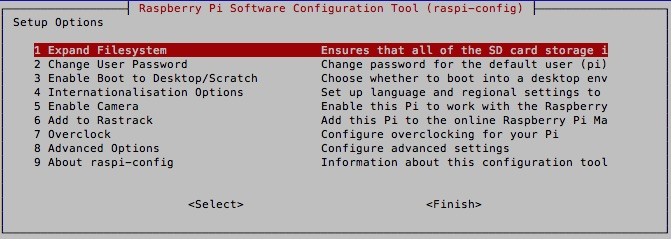
\includegraphics[width=15.8cm]{raspiconfig} \caption{siehe Punkt 7} \end{figure} Wählen Sie diesen aus und bestätigen im nächsten Menü die Eingabe, indem Sie \textit{Enable} auswählen. Nach einem Neustart ist die Raspberry Pi Kamera auch schon einsatzbereit. Ob die Kamera auch richtig funktioniert, können Sie mit dem Befehl \textit{"raspivid -t 0"} testen (Achtung: Bild wird nur bei direkt angeschlossenem Monitor angezeigt). 

\section{Der PIR-Sensor}
Der PIR-Sensor muss, im Gegensatz zur Kamera, ohne eigens dafür vorgesehenen Anschluss auskommen. Hierfür müssen wir auf die Pins des GPIO-Boards auf dem Raspberry Pi zugreifen. Allerdings sollte auch hier der Anschluss nicht viel Zeit in Anspruch nehmen. Zunächst sollte für Arbeiten am GPIO-Board generell der Strom am Raspberry Pi abgeschaltet sein, um einen Kurzschluss zu vermeiden. Für den Anschluss empfiehlt es sich außerdem, eine durchnummerierte Übersicht über die einzelnen Pins des GPIO-Boards des Raspberry Pi zur Hand zu haben. Je nach Modell unterscheidet sich die Belegung und die Anzahl der einzelnen Pins. Auf der Seite des Raspberry Pi benötigen wir einen 3,3 Volt-Pin, einen GPIO-Pin und einen Ground-Pin. Bei allen Raspberry Pi Modellen müssen wir für den GPIO-Pin den Pin mit der Nummer sieben wählen. Unser Programm wird auf genau diesen Pin horchen und durch Signaländerungen auf diesem Pin beeinflusst. \begin{figure}[h] \centering 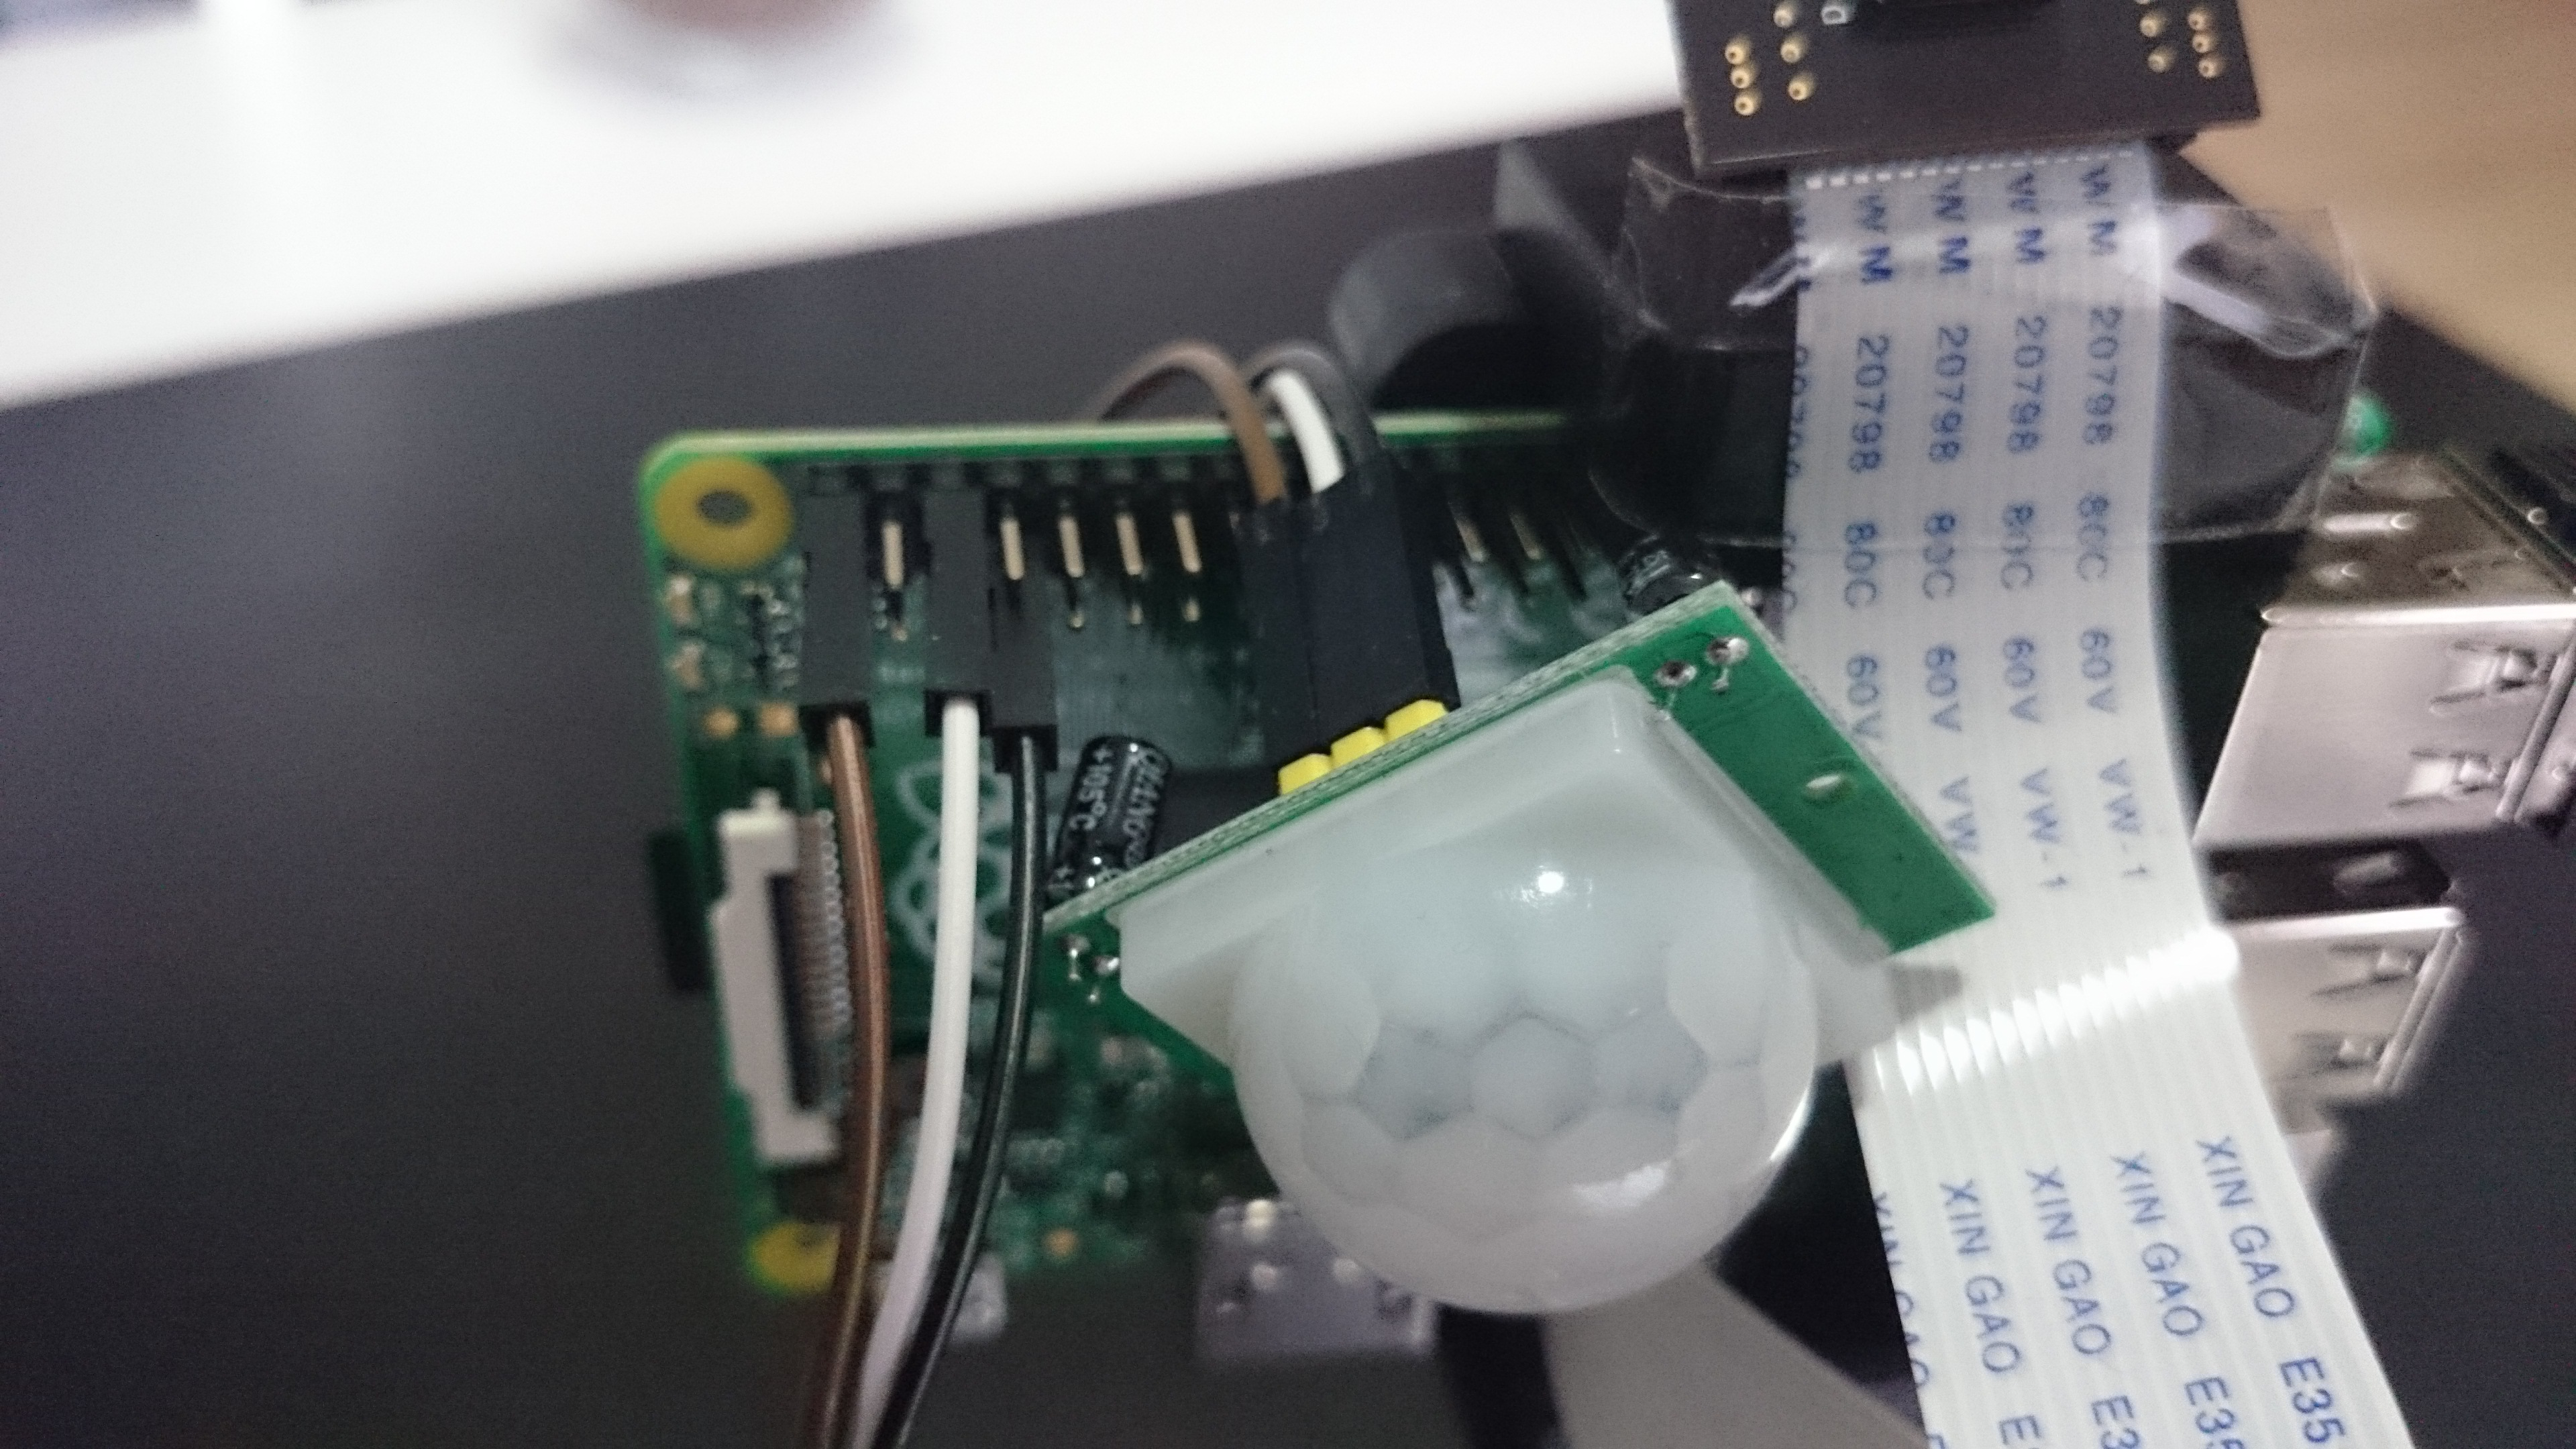
\includegraphics[width = 7.9cm]{pir1.JPG} \caption{Die Anschlüsse auf dem GPIO-Board} \end{figure} \begin{figure}[h] \centering 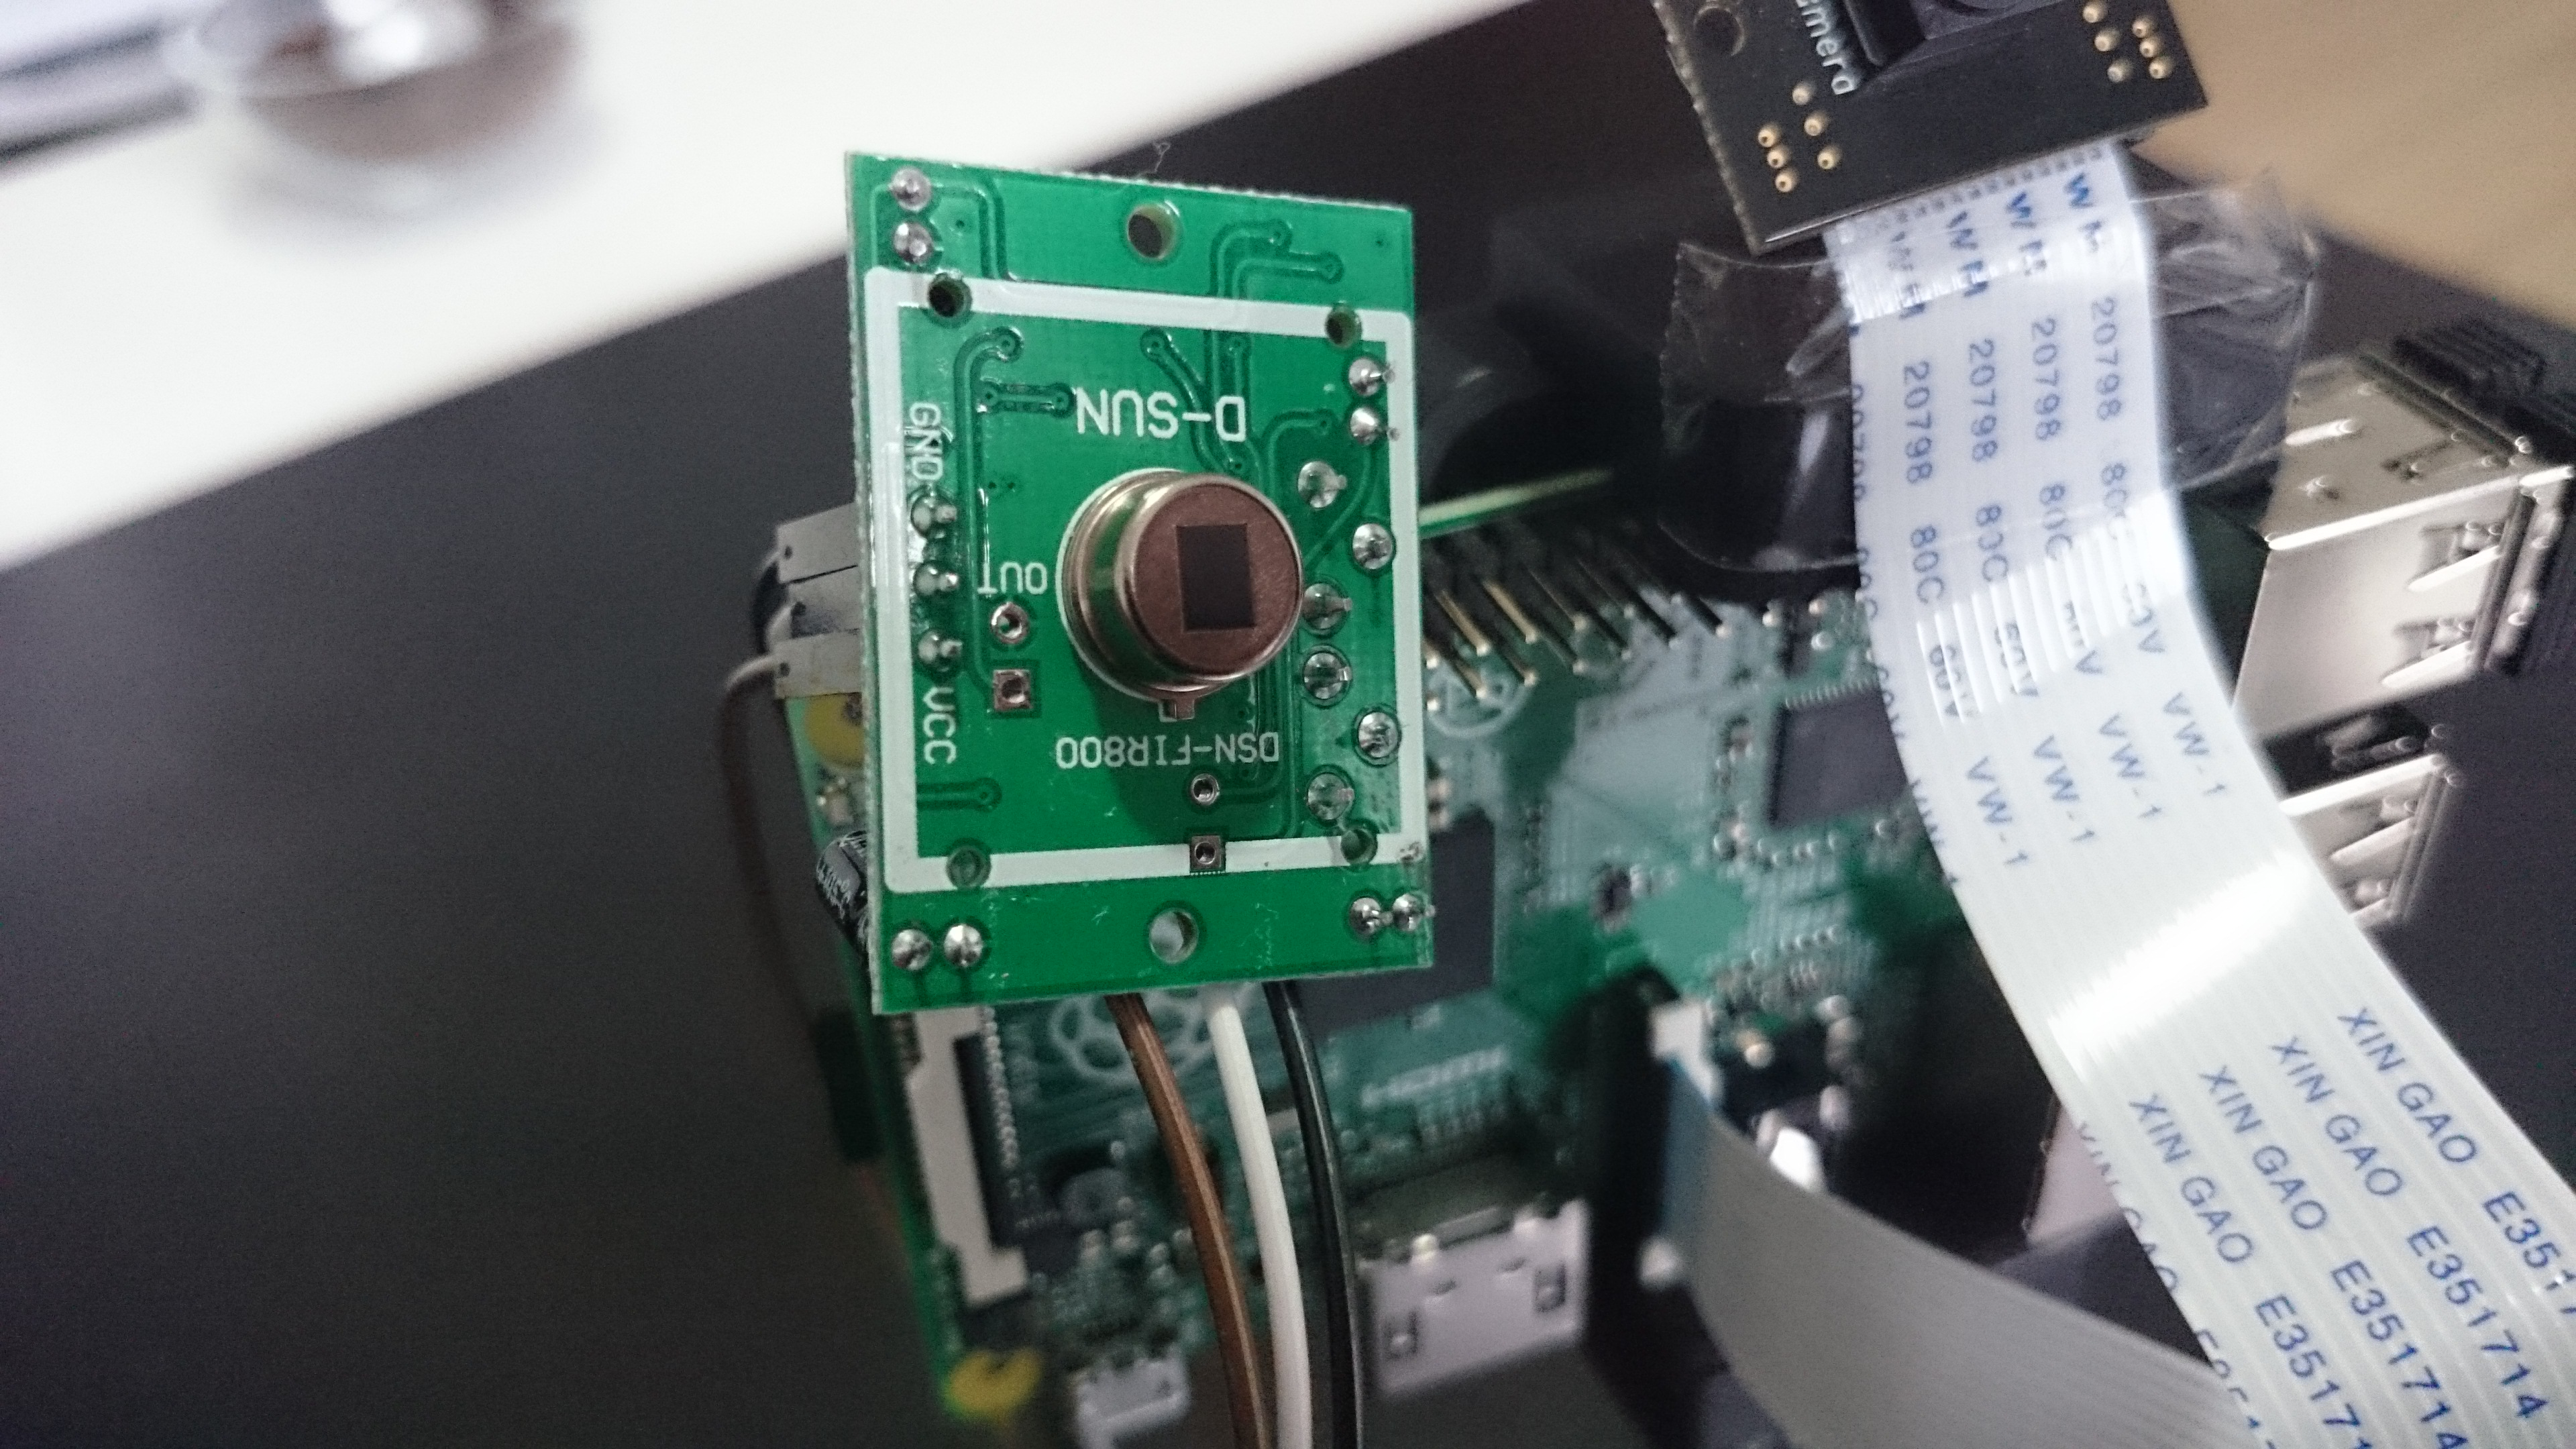
\includegraphics[width = 7.9cm]{pir2.JPG} \caption{Links sieht man gut die Beschriftung unter der Kuppel} \end{figure}Bei der Stromversorgung bleibt Ihnen die freie Wahl, wir schlagen allerdings Pin eins für die Stromversorgung mit 3,3 Volt und Pin sechs als Ground vor. Diese Konfiguration funktioniert auf allen Raspberry Pi Modellen. Um für den PIR-Sensor die jeweiligen Pins herauszufinden, müssen wir die milchige Kuppel auf dem Board des PIR-Sensors abziehen. Die Kuppel ist lediglich aufgesteckt und sollte leicht abzuziehen sein. Unter der Kuppel sehen wir, welcher Pin welchem Zweck dient. Stecken Sie nun die mit dem Raspberry Pi verbundenen Kabel auf ihre jeweiligen Gegenstücke auf dem Board des PIR-Sensors. Der Pin sechs vom GPIO-Board wird also auf den GND-Pin des PIR-Senors verbunden, Pin eins mit dem VCC-Pin des PIR-Sensors und Pin sieben mit dem mittleren OUT-Pin. Wenn Sie diese Schritte durchgeführt haben, können Sie den Raspberry Pi wieder mit dem Strom verbinden und hochfahren lassen. Ein Funktionstest ist jedoch nicht ohne Weiteres möglich, darauf müssen wir noch bis zur Inbetriebnahme der Software warten - oder Sie schreiben ein kleines Python-Script, dass die Funktion überprüft. Vergleichen Sie sonst Ihre Steckverbindungen mit der Abbildung 2.3.

\section{Die Handy-App}
Die Android-App, welche die Überwachungszentrale des Systems darstellt, kann bequem aus dem Google Play Store heruntergeladen werden und bedarf keiner weiteren Konfiguration. Sobald die App gestartet ist, ist diese auch bereits für den Empfang der Daten Ihrer Überwachungskamera(s) gerüstet.

\chapter{Das Programm}
\section{Das Programm starten}\todo[inline]{Vorgehen noch nicht final, Dateinamen eintragen}
Um das Programm auszuführen, navigieren Sie in das GIT-Repository dieses Projekts und laden die Datei namens "XXXX.py" herunter und speichern die Datei an einem leicht zugänglichen Ort. Öffnen Sie nun , falls noch nicht geschehen, das Terminal und navigieren Sie in den Ordner, in welchem die Datei abgelegt wurde. Um das Programm zu starten, müssen Sie dieses mit dem Befehl \textit{"sudo python3 XXXXX.py"} starten. Nun können wir die Funktionalität der Peripherie testen. Starten Sie jetzt zunächst die App auf Ihrem Handy oder dem Tablet. Die Software auf dem Raspberry Pi sollte zu diesem Zeitpunkt bereits die Kamera aktiviert haben. Ob dies der Fall ist, erkennen Sie anhand einer rot leuchtenden LED neben der Linse auf dem Kamera-Board. Falls dies nicht der Fall sein sollte, kontrollieren Sie, ob Sie die Kamera in der Konfiguration bereits aktiviert haben(siehe dazu Kapitel 1.5). Nun winken Sie in die Kamera und warten, ob sich der Prozentwert auf dem Handy oder dem Tablet ändert. Je länger die Bewegung dauert, umso höher steigt nun auch der Prozentwert in der App. Ob der PIR-Sensor ebenfalls in Betrieb ist, testen Sie indem Sie die Kamera nun kurz in eine andere Richtung Bewegen und nur der PIR-Sensor Sie erfassen kann. Ein wenig Eile ist hier gefragt, denn der PIR-Sensor ist nur für einige Sekunden in Betrieb, nachdem eine Bewegung von der Kamera erkannt wurde, um Energie einzusparen. Falls auch jetzt die Werte in der App steigen, ist auch der PIR-Sensor erfolgreich in Betrieb genommen worden.\\ \\Wenn Sie möchten, können Sie nun mit der Konfiguration eines weiteren Raspberry Pis beginnen. Falls Sie weitere Kameras aufbauen, müssen Sie an den bestehenden Systemen keine Änderungen vornehmen. Die Systeme kommunizieren automatisch miteinander, sofern sie sich im gleichen Netzwerk befinden. Wenn nun eines Ihrer Systeme eine Bewegung erkannt hat, erfahren die anderen Systeme dies automatisch und aktivieren ihre PIR-Sensoren, um nach einer Bewegung zu suchen. In den folgenden Tagen werden Sie die Möglichkeit zu schätzen lernen, per SSH auf Ihren Raspberry Pi zugreifen zu können. Je nach Positionierung des Überwachungssystems, könnte der Aufwand für das Auf- und Abbauen des Raspberry Pis mehr oder weniger aufwendig sein. Der Zugriff per SSH (oder VNC) erspart uns diese Arbeit und das starten und stoppen der Software, sowie das aktualisieren und nahezu alle anderen Tätigkeiten am Raspberry Pi, sind auch aus der Ferne möglich.

\section{Die Werte in der App}
Im Folgendem erklären wir kurz die Werte, die in der Begleitapp angezeigt werden. Die Werte ändern sich, wenn eine Bewegung erkannt worden ist. Je nach Dauer der Bewegung, klettert der Wert kontinuierlich nach oben. Die Kamera alleine lässt den Wert jede halbe Sekunde um fünf Prozent  steigen. Wenn der Wert also mehrere Sekunden lang steigt, ist auch mehrere Sekunden lang eine Bewegung durch die Kamera erkannt worden. Der PIR-Sensor funktioniert ähnlich, lässt den Wert allerdings um zehn Prozent pro halber Sekunde steigen. Der Wert ist höher, da die Wahrscheinlichkeit, dass eine Lebensform den Wert erhöht, sehr wahrscheinlich ist. Der PIR-Sensor reagiert nämlich lediglich auf die Wärmestrahlung eines bestimmten Infraroten Bereichs, welche von Menschen und Tieren ausgesendet wird. Fall Sie allerdings Ihre Einfahrt überwachen, sollten Sie sich darauf einstellen, dass auch Autos eine Infrarote Strahlung aussenden (es sei denn, der Motor ist noch kalt) und von dem PIR-Sensor dementsprechend bewertet werden. Falls sich also eine Wärmequelle an dem Sensor vorbei bewegt, erkennt der Sensor dies als Bewegung und erhöht den Wert in der App demgemäß. 


\end{document}